\documentclass[twocolumn]{article}

\usepackage{imr}
\usepackage{graphicx}
\usepackage{amsfonts}
\usepackage{bbm}       % for \mathbbm{1}
\usepackage{amsmath}
\usepackage{mathrsfs}  % for \mathscr
\usepackage{minted}    % for including source code
\usepackage{tikz}
\usetikzlibrary{decorations.markings}

\def\thepage {}
\bibliographystyle{imr}

\newenvironment{smallarray}[1]
 {\null\,\vcenter\bgroup\scriptsize
  \renewcommand{\arraystretch}{0.7}%
  \arraycolsep=.13885em
  \hbox\bgroup$\array{@{}#1@{}}}
 {\endarray$\egroup\egroup\,\null}

\begin{document}

\title{Linear-algebraic representation and transformation of unstructured meshes}
\author{Daniel Shapero$^1$}
\date{
    $^1$University of Washington, Seattle, WA, USA, shapero@uw.edu
}

\abstract{This paper will show some new approaches for implementing common transformations to the connectivity or topology of an unstructured mesh.
The key enabling technology for our approach is to borrow ideas from algebraic topology: we use the \emph{boundary operators} of a \emph{chain complex} to represent the mesh.
Boundary operators are really just integer matrices.
By representing the objects of study using the language of linear algebra, we can use linear algebraic reasoning and intuition to define transformations.}

\keywords{mesh generation, computational geometry, algebraic topology}

\maketitle
\thispagestyle{empty}
\pagestyle{empty}


% ====================
\section{Introduction}

Nearly all constructions in unstructured meshing require the ability to perform local transformations to the mesh topology.
For example, to compute the Delaunay triangulation, the Lawson algorithm uses a sequence of edge flips, while the Bowyer-Watson algorithm is based on splitting star-shaped polytopes along a vertex \cite{cheng2013delaunay}.
Algorithms for mesh coarsening, on the other hand, apply a sequence of edge or face collapses \cite{cignoni1998comparison}.
Implementing these low-level transformation kernels on common mesh data structures can be difficult and error-prone.
Are there other mesh data structures that make common algorithms easier to implement?

The idea of \emph{linear-algebraic representation} is to describe the mesh topology using a sequence of linear operators between certain vector spaces or modules.
The idea comes from algebraic topology: the linear operators are the \emph{boundary operators} on a certain \emph{chain complex}.
\textbf{If we can describe the mesh topology using linear algebra, then we can transform it using linear algebra as well.}
This viewpoint has been adopted in several publications on meshing and solid modeling \cite{dicarlo2007solid}, \cite{dicarlo2014linear}, \cite{mueller2017ternary}, \cite{paoluzzi2020topological}.
Other domains of science and engineering have seized on the idea of using linear algebra as the common language for building applications as well.
For example, the GraphBLAS project aims to implement common algorithms in graph theory using linear algebra \cite{mattson2013standards}.

This paper will show three transformations on the linear-algebraic represention of a polygonal mesh: (1) splitting a cell on a vertex, (2) merging adjacent cells, and (3) subdividing a cell along a collection of facets.
The main advantage of this linear-algebraic approach is that the transformation kernels are easy to write down and to code.
We show how other higher-level transformations can be implemented in terms of these primitive operations.
Finally, as a proof-of-concept, we implemented algorithms for computing convex hulls in arbitrary dimensions and constrained Delaunay triangulations in 2D.



% ==============
\section{Theory}

In this section, we will describe polytopal complexes, a class which includes all common types of meshes.
The boundary operators on a polytopal complex can be used as a data structure to represent the complex.
Next, we will describe how to convert between a polytopal complex and the more familiar representation of a simplicial complex as an array describing which vertices are contained in each simplex.
Finally, we'll then introduce the concept of a topological cone and give explicit formulae for the boundary operators of a cone.
The transformations that we describe in the next section all ``factor through'' the topological cone.

% ------------------------------
\subsection{Polytopal complexes}

We will assume as given the notions of simplices, cubes, polytopes, and meshes or spatial subdivisions made up of these objects.
The mathematical theory that underlies the rest of the paper is basic algebraic topology.
We will present very abbreviated definitions; we refer to \cite{dicarlo2007solid} for a longer exposition of the algebraic-topological point of view on solid modeling and to \cite{hatcher2002algebraic} for the theory of algebraic topology.

Let $\Omega$ be a polytopal mesh of some domain in Euclidean space.
Given a $k$-dimensional polytope $\sigma$ and a $k - 1$-dimensional face $\tau$ of $\sigma$, the \emph{incidence number} is an integer that describes the handedness or orientation with which $\tau$ is attached into $\sigma$.
We will write the incidence number as $[\sigma, \tau]$.
An informal definition of the incidence number is
\begin{equation}
    [\sigma, \tau] \equiv \begin{cases} +1 & \tau\text{ is attached positively in }\sigma \\ -1 & \tau\text{ is attached negatively in }\sigma \\ 0 & \tau\text{ is not in }\sigma\end{cases}.
\end{equation}
This informal definition is enough for the constructions that follow.
For example, if $e = \langle v_0, v_1\rangle$ is an edge connecting the vertices $v_0$ and $v_1$, then $[e, v_0] = -1$ and $[e, v_1] = +1$.
Likewise, if we consider a positively-oriented triangle $t = \langle v_0, v_1, v_2\rangle$, then the incidence number of $t$ to the edges $\langle v_0, v_1\rangle$, $\langle v_1, v_2\rangle$, and $\langle v_2, v_0\rangle$ are all positive.

% TODO: Add labels to the figure and the boundary matrices, see
% https://tex.stackexchange.com/a/59732
\begin{figure}[t]
    \begin{minipage}{0.48\linewidth}
        \begin{center}
            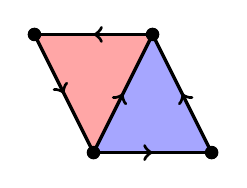
\begin{tikzpicture}[scale=0.75]
    \coordinate (p1) at (1, 0){};
    \coordinate (p2) at (3, 0){};
    \coordinate (p3) at (2, 2){};
    \coordinate (p4) at (0, 2){};

    \draw[fill=blue!35] (p1) -- (p2) -- (p3) -- cycle;
    \draw[fill=red!35] (p1) -- (p3) -- (p4) -- cycle;
    \begin{scope}[
        very thick,
        decoration={markings, mark=at position 0.5 with {\arrow{>}}}
    ]
        \draw[postaction={decorate}] (p1) -- (p2);
        \draw[postaction={decorate}] (p2) -- (p3);
        \draw[postaction={decorate}] (p3) -- (p4);
        \draw[postaction={decorate}] (p4) -- (p1);
        \draw[postaction={decorate}] (p1) -- (p3);
    \end{scope}
    \foreach \p in {p1, p2, p3, p4} {
        \filldraw (\p) circle (3pt);
    }
\end{tikzpicture}


        \end{center}
    \end{minipage}
    \hfill
    \begin{minipage}{0.48\linewidth}
        {\small
            \begin{equation*}
                \partial_1 = \left[\begin{smallmatrix}
                    - &   & + & - &   \\
                    + & - &   &   & + \\
                      & + & - &   &   \\
                      &   &   & + & -
                \end{smallmatrix}\right]
            \end{equation*}
            \begin{equation*}
                \partial_2 = \left[\begin{smallmatrix}
                    \textcolor{red!65}+ & \textcolor{blue!65}- \\
                    \textcolor{red!65}+ &   \\
                    \textcolor{red!65}+ &   \\
                      & \textcolor{blue!65}+ \\
                      & \textcolor{blue!65}+
                \end{smallmatrix}\right]
            \end{equation*}
        }
    \end{minipage}
    \caption{Pair of adjacent triangles (left) and their boundary matrices (right).}
    \label{fig:two-triangle-chain-complex}
\end{figure}

Let $n_k$ be the number of cells of $\Omega$ of dimension $k$.
Suppose additionally that we have numbered all of the $k - 1$-cells as $\{\tau_i\}_{i = 1}^{n_{k - 1}}$ and the $k$-cells as $\{\sigma_j\}_{j = 1}^{n_k}$.
The $k$-th boundary matrix $\partial_k$ is an integer matrix of size $n_{k - 1} \times n_k$.
The $i, j$ entry of this matrix is
\begin{equation}
    (\partial_k)_{ij} = [\sigma_j, \tau_i].
\end{equation}
These operators act on certain spaces of \emph{chains} but the theory behind this will not be important for the following.
By reading off columns of each boundary matrix, we can quickly determine which $k - 1$-cells are faces of a given $k$-cell and how they are attached.
To continue with the example above, we might say that if $e = \langle v_0, v_1\rangle$ is an edge, then $\partial e = +v_1 - v_0$.
Likewise, if $t = \langle v_0, v_1, v_2\rangle$ is a triangle, then $\partial t = \langle v_0, v_1\rangle + \langle v_1, v_2\rangle + \langle v_2, v_0\rangle$.
Figure \ref{fig:two-triangle-chain-complex} shows the boundary matrices for two adjacent triangles.

\textbf{The most important fact about boundary operators is that the boundary of a boundary is always equal to zero:}
\begin{equation}
    \partial_k\cdot\partial_{k + 1} = 0.
    \label{eq:ddzero}
\end{equation}
This relation has to be proved in each case from certain basic facts about incidence numbers.
For formal proofs, see \cite{hatcher2002algebraic} for the simplicial case and \cite{massey2019basic} for the cubical and general cases.

There is one final definition that will clarify a later construction at a critical juncture.
The definitions above assume that the mesh terminates at the points or 0-dimensional cells.
We will instead include a single \emph{bottom} cell $\bot$ of dimension $-1$ and we will say that the bottom cell is positively incident to every vertex, i.e.
\begin{equation}
    [v, \bot] = +1
\end{equation}
for all vertices $v$.
We can then define the 0-boundary operator $\partial_0$ as a row vector of all 1s:
\begin{equation}
    \partial_0 = \mathbbm{1}^*.
    \label{eq:0-boundary-matrix}
\end{equation}
The condition that $\partial_0\partial_1 = 0$ now implies that the boundary of every edge has one positive and one negative vertex: $\partial e = v_i - v_j$ for some $i$, $j$.
We cannot have that, say, $\partial e = v_i + v_j$.
This outcome would be undesirable but we have not explicitly forbidden it otherwise.
Equation \eqref{eq:0-boundary-matrix} will reappear when we define the split transformation.

The boundary matrices do not capture important geometric data describing how cells are embedded into Euclidean space.
We could have the same connectivity structure for two different triangular meshes, one which uses only piecewise linear facets and another that uses curved polynomial mappings.
In the remainder, we consider only transformations to the connectivity structure or topology and not to the geometry.

What kinds of alterations or transformations to a set of boundary matrices preserve the fundamental relation $\partial\partial = 0$?
Suppose $A$, $B$ are integer matrices, $\{\partial_0, \ldots, \partial_n\}$ are boundary matrices, and we define
\begin{equation}
    \partial_k' = \partial_k\cdot A, \quad \partial_{k + 1}' = B\cdot\partial_{k + 1}.
\end{equation}
What conditions do we need on $A$ and $B$ in order to guarantee that $\partial_k'\cdot\partial_{k + 1}' = 0$?
One sufficient condition is that \emph{the image of $\partial_{k + 1}$ is an invariant subspace of $A\cdot B$}.
An important particular case is $A\cdot B = I$, which includes both permutations and sign flips.
We can reorder the columns of $\partial_k$ so long as we apply the inverse permutation to the rows of $\partial_{k + 1}$.
Likewise, we can flip the sign of any column of $\partial_k$ as long as we flip the sign of the corresponding row of $\partial_{k + 1}$.
Speaking informally, we can say that individual incidence numbers don't matter as much as the relation between all cells and faces.
The more general case where $A\cdot B$ is not equal to the identity matrix but its image is an invariant subspace of $\partial_{k + 1}$ is needed for other transformations, such as merging multiple cells into one or deleting cells.

\subsection{Simplicial complexes}

For many problems in meshing, the goal is to produce a mesh where all the cells are simplices or cubes rather than general polytopes.
The utility of polytopal meshes is that they can represent intermediate states that are not of the right type.
For example, one might merge a set of triangles into a polygon and then split or subdivide the polygon into a different triangulation incrementally.
A polytopal mesh can represent the polygonal intermediate states, whereas if one could only represent triangular data then this transformation has to be completed all in one shot.
But the ability to use polytopal meshes, or more specifically the boundary operators, as an intermediate step relies on the ability to convert between the two.

We assume that the standard data structure for a pure, orientable $k$-dimensional simplicial complex is an array of size $n \times (k + 1)$ where $n$ is the number of top simplices.
Each row of this array stores the vertices of the corresponding simplex, ordered in such a way to give a positive orientation.
For a $k$-dimensional complex embedded in $\mathbb{R}^k$, positive orientation is the usual condition that the determinant of the matrix formed by a simplex's points in homogeneous coordinates is positive.
The order is non-unique up to any permutation with positive parity.

\textbf{Simplicial $\rightarrow$ polytopal}.
Let $\sigma = \langle v_0, \ldots, v_k\rangle$ be an oriented $k$-simplex.
If we re-order the vertices of $\sigma$ by some permutation $p$, then we get the same simplex if $p$ has positive parity and the ``opposite'' simplex if $p$ has negative parity:
\begin{equation}
    \langle v_{p(0)},\ldots,v_{p(k)}\rangle = \text{parity}(p)\cdot\langle v_0,\ldots, v_k\rangle
\end{equation}
The incidence number from $\sigma$ to the face $\tau = \langle v_0, \ldots, \hat v_j, \ldots, v_k\rangle$ obtained by removing the $j$th vertex is positive if $j$ is even and negative if $j$ is odd, or
\begin{equation}
    [\sigma, \tau] = (-1)^j.
    \label{eq:simplicial-incidence-numbers}
\end{equation}
We can motivate this formula by observing that if $\sigma$ is in $\mathbb{R}^k$, the oriented half-space formed by the $j$th face contains $\sigma$ if $j$ is even and does not contain $\sigma$ if $j$ is odd.
Given a numbering scheme for all the simplices of the mesh, the previous equation gives us the incidence numbers that we need to fill in the entries of the boundary matrices for each simplex.

\textbf{Polytopal $\rightarrow$ simplicial}.
Suppose that $\{\partial_0, \ldots, \partial_k\}$ are the boundary operators of a single simplex with vertices $v_0, \ldots, v_k$.
We do not know whether the right order of the vertices is $\langle v_0,\ldots,v_k\rangle$ or some orientation-reversing permutation.
Now let $\{\partial_0',\ldots,\partial_k'\}$ be the boundary matrices of a simplex using the canonical choice of incidence numbers from equation \eqref{eq:simplicial-incidence-numbers}.
The goal is to find an isomorphism of the two complexes.
We take the starting permutation and sign flip matrices to be $P_0 = I_{n_0}$ where $n_0$ is the number of vertices and $s_0 = \mathbbm{1}$.
For each dimension $1 \le j < k$, we find a permutation matrix $P_j$ and sign flips $s_j$ such that
\begin{equation}
    \text{diag}(s_{j - 1})\cdot P_{j - 1}^*\cdot\partial_j \cdot P_j\cdot \text{diag}(s_j) = \partial_j'.
\end{equation}
The permutations can be found by finding columns with the same sets of non-zero entries.
Finally, at dimension $k$, we will find that $\text{diag}(s_{k - 1})\cdot P_{k - 1}^*\partial_k$ is a column vector of all +1 or -1.
If the resulting vector is positive, then the ordering $\langle v_0,\ldots,v_k\rangle$ will result in boundary matrices that are isomorphic to the input boundary matrices.
Otherwise, any orientation-reversing permutation of that order is the correct choice.
We can then apply this logic to each top-dimensional cell of a whole complex provided that it is known to be simplicial.
If at any point a set of permutations and sign flips cannot be found, the resulting polytopal complex was not simplicial.

% ----------------------
\subsection{Cone spaces}

In the next section, we will show several transformations on a polytopal complex that are expressible as operations on their boundary matrices.
Each of these transformations is a type of \emph{bistellar move}, also referred to in the literature as a Pachner move after U. Pachner \cite{pachner1990shellings, pachner1991pl, casali1995note}.
A bistellar move of a set of cells of a mesh first embeds them into the boundary of a higher-dimensional ball, and then replaces them with the closure of their complement in the boundary of the ball.
These transformations are known to preserve important invariants and other global properties.
The fact that the new cells have the same boundary as the old ensures that the the fundamental relation $\partial\partial = 0$ is preserved.
But how we polygonize the higher-dimensional ball is a matter of choice.
The constructions that follow are all based on a particular polygonization called the topological \emph{cone}.

\begin{figure}[t]
    \begin{center}
        \includegraphics[width=0.9\linewidth]{figures/cone.pdf}
    \end{center}
    \caption{A 2D footprint polygon (left) and its topological cone (right).}
    \label{fig:cone}
\end{figure}

To describe what a topological cone is, it is helpful to first describe the concept of a \emph{join}.
The join of two subsets $C$ and $C'$ of Euclidean space is the set
\begin{equation}
    C * C' = \{\lambda\cdot c + (1 - \lambda)c' : c \in C, c' \in C', \lambda \in [0, 1]\}.
\end{equation}
Intuitively, the join of two spaces consists of the set of all lines between them.
If $C$ and $C'$ are, respectively, $m$- and $n$-dimensional submanifolds, then $C * C'$ is $m + n + 1$-dimensional.
An important fact for the transformations that we'll define is that the join of an $m$-simplex and an $n$-simplex is an $m + n + 1$-simplex.

The topological cone of a space $\Omega$, which we will write as $\text{cone}(\Omega)$, is the join with a single point.
We will refer to this added point as the \emph{apex}.
An illustration is shown in Figure \ref{fig:cone}.
Suppose that we have a set of boundary matrices $\{\partial_0, \ldots, \partial_n\}$ for a space $\Omega$.
\textbf{We can express the boundary matrices $\{\partial_0', \ldots, \partial_{n + 1}'\}$ for $\text{cone}(\Omega)$ in terms of the boundary matrices of the original space.}
This construction underlies both the vertex- and face-split transformations described below.

First, if the original space has $N$ vertices, the cone space adds one more.
So $\partial_0$ is a row vector of all 1s with $N$ columns, and $\partial_0'$ is a row vector of all 1s with $N + 1$ columns.
Next, the cone space includes all the 1-cells or edges of the original space, so we know that $\partial_1'$ will include $\partial_1$ as a sub-matrix.
Forming the cone space adds edges between every original vertex and the apex of the cone.
Any one of these edges could have negative or positive incidence on the apex.
But by applying sign flips to the columns of $\partial_1'$, which as per the previous section does not alter the topology, we can always guarantee that every edge has positive incidence to an original vertex and negative incidence to the new cone vertex.
In linear algebraic terms,
\begin{equation}
    \partial_1' = \left[\begin{matrix}\partial_1 & I \\ 0 & -\mathbbm{1}^*\end{matrix}\right]
\end{equation}
where $\mathbbm{1}$ is the vector of all 1s.
Moreover, we can observe here that the row vector of all 1s is the same as the 0-boundary matrix:
\begin{equation}
    \partial_1' = \left[\begin{matrix}\partial_1 & I \\ 0 & -\partial_0\end{matrix}\right].
    \label{eq:cone-partial1}
\end{equation}
We can then state that the number of edges or 1-cells in the cone space is equal to $\#\text{vertices} + \#\text{edges}$.

Now we need to determine what the remaining boundary operators should be.
We can start by counting how many 2-cells there should be in the cone.
Every 2-cell of the original space must also be present in the cone.
The added 2-cells are formed through a topological join of the original 1-cells with the cone vertex.
So we can again state that the number of 2-cells in the cone space is equal to $\#\text{2-cells} + \#\text{1-cells}$.
Again, in principle all of the new 2-cells could have a completely arbitrary incidence w.r.t. to the original 1-cells, but by a sign flip we can ensure instead that all of these incidences are positive.
In other words, so far, we know that the 2-boundary matrix has the form
\begin{equation}
    \partial_2' = \left[\begin{matrix}\partial_2 & I \\ 0 & [?]\end{matrix}\right]
\end{equation}
where the question mark is a matrix that has to be determined.
We have a constraint, however, that $\partial_1'\cdot\partial_2' = 0$.
The upper-right block of the product $\partial_1'\cdot\partial_2'$ is
\begin{equation}
    \partial_1\cdot I + I\cdot [?]
\end{equation}
and a solution that would make this expression equal to zero is to take $[?] = -\partial_1$.
In other words, we make the ansatz
\begin{equation}
    \partial_2' = \left[\begin{matrix}\partial_2 & I \\ 0 & -\partial_1\end{matrix}\right].
    \label{eq:cone-partial2}
\end{equation}
Calculating each block by hand, we find that this guess does indeed make $\partial_1'\cdot\partial_2' = 0$.

Equations \eqref{eq:cone-partial1} and \eqref{eq:cone-partial2} both have the same form but with the dimensions incremented by 1.
We can then guess that, in general, all of the boundary matrices of the cone space up to dimension $n$ have the form
\begin{equation}
    \partial_k' = \left[\begin{matrix}\partial_k & I \\ 0 & -\partial_{k - 1}\end{matrix}\right].
    \label{eq:cone-partial-k}
\end{equation}
Again, a rudimentary hand-computation by blocks shows that $\partial_k'\cdot\partial_{k + 1}' = 0$.
To complete the construction, the final boundary matrix is
\begin{equation}
    \partial_{n + 1}' = (-1)^n\left[\begin{matrix}-I \\ \partial_n\end{matrix}\right].
    \label{eq:cone-partial-n+1}
\end{equation}
We will explain the sign convention below.
\textbf{These two equations are the crux of the paper.}

A few consequences of equations \eqref{eq:cone-partial-k}, \eqref{eq:cone-partial-n+1} are then apparent.
First, the number of $k$-cells in $\text{cone}(\Omega)$ is equal to the number of $k$-cells + the number of $k - 1$-cells in $\Omega$.
Second, while we have chosen particular signs for the incidence numbers, we can flip these signs as we see fit.
For example, in the vertex-split transformation we will write the $n$-boundary matrix as
\begin{equation}
    \partial_n' = \left[\begin{matrix}\partial_n & \text{diag}(\partial_n\cdot\mathbbm{1}) \\ 0 & -\partial_{n - 1}\cdot\text{diag}(\partial_n\cdot\mathbbm{1})\end{matrix}\right]
\end{equation}
with an equivalent sign flip applied to the $n + 1$-boundary matrix.
Finally, we can write down a formula for the boundary matrices of the \emph{suspension} of a space -- the topological join with two isolated points instead of one -- in the same way:
\begin{equation}
    \partial_{k + 1}' = \left[\begin{matrix}\partial_k & I & I \\ 0 & -\partial_{k - 1} & 0 \\ 0 & 0 & -\partial_{k - 1}\end{matrix}\right]
    \label{eq:suspension-partial-k}
\end{equation}
and for the top cells
\begin{equation}
    \partial_{n + 1}' = (-1)^n\left[\begin{matrix}-I & +I \\ +\partial_n & 0 \\ 0 & -\partial_n\end{matrix}\right].
    \label{eq:suspension-partial-n+1}
\end{equation}
Suspensions will appear again when we consider 2-3 flips of tetrahedra and multi-face retriangulation.

Before we proceed to the transformations themselves, we should explain the sign convention in equation \eqref{eq:cone-partial-n+1}.
The sign of the final boundary matrix is ultimately arbitrary -- we can multiply on the right by any sign flip and still preserve $\partial\partial = 0$.
But we can pick a normalization by the following argument.
The standard construction defines the boundary of a $k$-simplex according to equation \eqref{eq:simplicial-incidence-numbers}.
But we can also construct the simplex inductively as a cone space.
A 0-simplex is a single point, and a $k + 1$-simplex is the cone of a single point and the $k$-simplex with boundary matrices chosen according to equations \eqref{eq:cone-partial-k} and \eqref{eq:cone-partial-n+1}.
Choosing the normalization factor $(-1)^n$ makes the repeated cone construction isomorphic to the positively-oriented simplex through a sequence of permutations and sign flips.
With no normalization at all, the even-dimensional simplices under the cone construction are instead isomorphic to the standard construction \emph{but with the opposite orientation}.

The constructions above are not new.
Equation \eqref{eq:cone-partial-k} has appeared before in the literature on homological algebra \cite{gelfand1994homological}.
The simpcomp package of the GAP system includes routines for computing topological cones of abstract simplicial complexes and for performing bistellar moves \cite{bjorner2000simplicial, effenberger2011simpcomp}.
The polymake library also includes routines for bistellar moves \cite{gawrilow2000polymake}.
Both simpcomp and polymake include these features for determining when two simplicial complexes are piecewise linear-homeomorphic, not for computational meshing.
The utility of the topological cone for computational meshing, which we demonstrate below, has not appeared elsewhere as far as we know.


% =======================
\section{Transformations}

Having written down the explicit formulas \eqref{eq:cone-partial-k} and \eqref{eq:cone-partial-n+1} for the boundary matrices of a cone, we can then apply them to define transformations.

% ------------------
\subsection{Merging}

A \emph{merge} of a set of $k$-cells replaces them with a single cell (provided that their union is simply-connected).
Merging is a column operation on the matrix $\partial_k$.
In the simplest case, the result column is the sum of all the columns to be merged, but in general we might need to flip some signs:
\begin{align}
    \partial_k' & = \partial_k\cdot\text{diag}(s_0, \ldots, s_m)\cdot\mathbbm{1}, \\
    \partial_{k + 1}' & = \left[\begin{matrix} 0 \ldots 1 \ldots 0\end{matrix}\right]\partial_{k + 1}. \label{eq:merge-k+1}
\end{align}
where $s_i$ are all $\pm 1$.
The signs are chosen so that any higher-dimensional cell $\sigma$ has the same incidence with respect to any of the cells $\tau$ to be merged.
The transformation to the rows of $\partial_{k + 1}$ collapses all incidence to any of the desired $k$-cells into incidence to the merged $k$-cell.
For merging cells of top dimension $n$, there are no higher-dimensional cells to apply equation \eqref{eq:merge-k+1} to and this step is left out.

\emph{Edge collapsing}, the key transformation in surface simplification algorithms \cite{gueziec1995surface}, is a merge of two vertices.

% ---------------------------
\subsection{Vertex-splitting}

A \emph{vertex-split} divides the union of several polytopes along a vertex.
The key correctness criteria for this operation are that (1) every newly-created polytope contains the splitting vertex and (2) the boundary of the sum of all polytopes does not change.
This second condition can be expressed mathematically as
\begin{equation}
    \partial_n'\cdot\mathbbm{1} = \left[\begin{matrix}\partial_n\cdot\mathbbm{1} \\ 0\end{matrix}\right].
    \label{eq:split-preserves-boundaries}
\end{equation}
The cells of the vertex split can be obtained as the ``top'' of the topological cone of the original cells, so equations \eqref{eq:cone-partial-k} and \eqref{eq:cone-partial-n+1} are applicable with some modifications.
Boundary matrices $\partial_0'$ through $\partial_{n - 1}'$ all transform according to equation \eqref{eq:cone-partial-k}.

For dimension $n$, we want to do three things differently.
First, the cone over a space has 1 higher dimension, but we want to transform a space to one of the same dimension.
We thus discard the $n + 1$-th boundary matrix from the cone when we form a vertex split.
Second, the cone over a space includes the space itself as a sub-complex, whereas we want to remove the original polytopes.
The resulting modification is that we discard the lower- and upper-left blocks of $\partial_n'$ from the usual formula for cones.
Finally, we want to preserve the original boundary of the starting polytopes, as specified in equation \eqref{eq:split-preserves-boundaries}.
The alteration to the usual cone formula is to multiply $\partial_n'$ on the right by the diagonal matrix $\text{diag}(\partial_n\cdot\mathbbm{1})$.
Putting all of these together, we find that
\begin{align}
    \partial_n' & \equiv \left[\begin{matrix}\partial_n & I \\ 0 & -\partial_{n - 1}\end{matrix}\right]\cdot \underbrace{\left[\begin{matrix}0 \\ I\end{matrix}\right]}_{\text{cut left}\atop\text{column}}\cdot \underbrace{\text{diag}(\partial_n\cdot\mathbbm{1})}_{\text{preserve}\atop\text{boundaries}} \nonumber\\
        & = \left[\begin{matrix}\text{diag}(\partial_n\cdot\mathbbm{1}) \\ -\partial_{n - 1}\cdot\text{diag}(\partial_n\cdot\mathbbm{1})\end{matrix}\right]
    \label{eq:vertex-split-n}
\end{align}
We can see that this choice of $\partial_n'$ satisfies equation \eqref{eq:split-preserves-boundaries} by using the fact that $\text{diag}(z)\cdot\mathbbm{1} = z$ for any vector $z$.

A final pruning step is necessary when we split the union of more than one polytope.
The vector $\partial_n\cdot\mathbbm{1}$ will have zero entries along any interior faces.
Consequently, some $n - 1$-cells of the newly-generated complex are not in the boundary of any $n$-cell.
We can then remove these zero rows from $\partial_n'$ and columns from $\partial_{n - 1}'$.
Proceeding down by dimension, we remove any row from $\partial_k'$ that is all zeros and the corresponding column from $\partial_{k - 1}'$ for $k = n - 1, \ldots, 1$.

Figure \ref{fig:split-transformation} illustrates the split transformation on a single quadrilateral and shows the boundary matrices before and after.
The Bowyer-Watson algorithm for computing Delaunay triangulations and all common algorithms for computing convex hulls require only the vertex-split transformation \cite{cheng2013delaunay}.

\begin{figure}[h]
    \begin{center}
        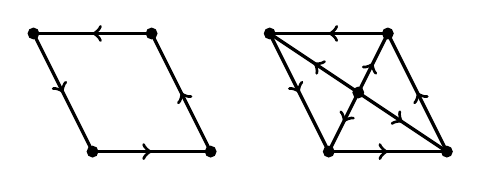
\begin{tikzpicture}[scale=0.75]
    \newcommand*{\defcoords}{
        \coordinate (p0) at (1.5, 1){};
        \coordinate (p1) at (1, 0){};
        \coordinate (p2) at (3, 0){};
        \coordinate (p3) at (2, 2){};
        \coordinate (p4) at (0, 2){};
    }

    \begin{scope}[
        very thick,
        decoration={markings, mark=at position 0.5 with {\arrow{>}}}
    ]
        \defcoords
        \draw[postaction={decorate}] (p1) -- (p2);
        \draw[postaction={decorate}] (p2) -- (p3);
        \draw[postaction={decorate}] (p3) -- (p4);
        \draw[postaction={decorate}] (p4) -- (p1);

        \foreach \p in {p1, p2, p3, p4} {
            \filldraw (\p) circle (2pt);
        }
    \end{scope}

    \begin{scope}[
        very thick,
        shift={(4, 0)},
        decoration={markings, mark=at position 0.5 with {\arrow{>}}}
    ]
        \defcoords
        \draw[postaction={decorate}] (p1) -- (p2);
        \draw[postaction={decorate}] (p2) -- (p3);
        \draw[postaction={decorate}] (p3) -- (p4);
        \draw[postaction={decorate}] (p4) -- (p1);
        \draw[postaction={decorate}] (p0) -- (p2);
        \draw[postaction={decorate}] (p0) -- (p3);
        \draw[postaction={decorate}] (p0) -- (p4);
        \draw[postaction={decorate}] (p0) -- (p1);

        \foreach \p in {p0, p1, p2, p3, p4} {
            \filldraw (\p) circle (2pt);
        }
    \end{scope}
\end{tikzpicture}


    \end{center}

    \begin{equation*}
        \partial_1 = \left[\begin{smallmatrix}
            - &   &   & + \\
            + & - &   &   \\
              & + & - &   \\
              &   & + & -
        \end{smallmatrix}\right],
        \quad
        \partial_2 = \left[\begin{smallmatrix}
            + \\ + \\ + \\ +
        \end{smallmatrix}\right]
    \end{equation*}

    \begin{equation*}
        \partial_1' = \left[\begin{smallarray}{cccc|cccc}
            - &   &   & + & + &   &   &   \\
            + & - &   &   &   & + &   &   \\
              & + & - &   &   &   & + &   \\
              &   & + & - &   &   &   & + \\
            \hline
              &   &   &   & - & - & - & -
        \end{smallarray}\right], \quad
        \partial_2' = \left[\begin{smallarray}{cccc}
            + &   &   &   \\
              & + &   &   \\
              &   & + &   \\
              &   &   & + \\
            \hline
            + &   &   & - \\
            - & + &   &   \\
              & - & + &   \\
              &   & - & +
        \end{smallarray}\right]
    \end{equation*}

    \caption{Quadrilateral before and after splitting on a new vertex in the center (top) and boundary matrices before and after (bottom).}
    \label{fig:split-transformation}
\end{figure}

% -------------------------
\subsection{Face-splitting}

A \emph{face-split} divides a polytope into several cells along a collection of splitting faces.
We assume that the initial polytope is not incident upon the splitting faces.
The correctness criteria for this operation are that (1) each new polytope is incident on the splitting faces and (2) the boundary of the sum of all polytopes does not change.

In order to be able to split the top cell, we need to assume a certain connectivity structure between its faces.
A $k$-\emph{path} in $\Omega$ is a collection $\{f_0, s_0, f_1, s_1, \ldots, f_{m - 1}, s_{m - 1}, f_m\}$ such that $s_i$ is a $k - 1$-face of both $f_i$ and $f_{i + 1}$ for each $i$.
Given two collections of $k$-cells $F_1$, $F_2$, we say that a third collection of $k$-cells $F$ is a \emph{separator} for $F_1$, $F_2$ if any path from a cell $f_1$ in $F_1$ to a cell $f_2$ in $F_2$ must pass through a $k - 1$-face $s$ of some $f$ in $F$.
The definition is similar to that of graph theory but with some important differences in the case of polytopal complexes.

In order to be able to subdivide $P$ into multiple cells, we need to be able to partition its faces into two or more groups $\{F_1, \ldots, F_m\}$ with a common separator $F_0$.
Moreover, we assume at first that $[P, F_0] = 0$ and $[P, F_i] \neq 0$ for $i \ge 1$.
We can find separators and subgroups through a procedure analogous to breadth-first search but with adjacency defined by sharing common subfaces.

The $n - 1$-boundary matrix will have the form
\begin{equation}
    \partial_{n - 1} = \Big[\begin{matrix}[S, F_0] & [S, F_1] & \cdots & [S, F_m]\end{matrix}\Big],
\end{equation}
where $S$ denotes the set of all subfaces or $n - 2$-dimensional cells contained in $P$, and
\begin{equation}
    \partial_n = \left[\begin{matrix} 0 \\ [F_1, P] \\ \vdots \\ [F_m, P]\end{matrix}\right].
\end{equation}
The fundamental equation \eqref{eq:ddzero} then implies that
\begin{equation}
    \sum_i[S, F_i]\cdot[F_i, P] = 0.
    \label{eq:face-split-ddzero}
\end{equation}
We will not alter the $n - 1$-boundary matrix at all, only the $n$-boundary matrix.

Now we make the ansatz that the transformed $n$-boundary matrix will have one column for each connected component; each column will have one block for the separator $F_0$; and column $k$ will have a non-zero block for the corresponding component $F_k$.
In all, the new matrix will have the form
\begin{equation}
    \partial_n' = \left[\begin{matrix}[F_0, P_1] & \cdots & [F_0, P_m] \\ [F_1, P] & & \\ & \ddots & \\ & & [F_m, P]\end{matrix}\right]
\end{equation}
where the incidences $[F_0, P_i]$ need to be solved for.
The incidences $[F_i, P]$ are the same as in the initial polytope.
If we can show that $\sum_i[F_0, P_i]\mathbbm{1} = 0$, then the boundary of the new polytopes will be the same as the old.
To preserve the fundamental equation $\partial\partial = 0$, we need that
\begin{equation}
    [S, F_0][F_0, P_i] = -[S, F_i][F_i, P]
\end{equation}
for each $i$.
We can then attempt to find a solution of this collection of linear systems of equations.
The existence of a solution is not guaranteed a priori, but if we can find one then it defines a valid subdivision of the original cell.
The system is also rectangular, so it may be under- or over-determined depending on the number of faces and subfaces.
We can obtain a square system by instead opting to solve
\begin{equation}
    [S, F_0]^*[S, F_0][F_0, P_i] = -[S, F_0]^*[S, F_i][F_i, P].
    \label{eq:face-split-normal-eqn}
\end{equation}
We can compute solutions to integer linear systems by first finding the Hermite normal form of the system matrix \cite{kannan1979polynomial}.
Let $[S, F_0]^+$ denote the pseudo-inverse of this system or the matrix $\{[S, F_0]^*[S, F_0]\}^{-1}[S, F_0]$ if the system is solvable.
Then
\begin{align}
    & \sum_i[F_0, P_i]\mathbbm{1} = \nonumber\\
    & \quad\quad -[S, F_0]^+\sum_i[S, F_i][F_i, P]
\end{align}
which equals zero by equation \eqref{eq:face-split-ddzero}, so indeed the new polytopes have the same boundary as the old.

We can also look at this transformation as a bistellar move.
Both the old polytope and the new polytopes are the common boundary of the $n + 1$-polytope with boundary matrices
\begin{equation}
    \partial_n' = \left[\begin{matrix}0 & [F_0, P_1] & \cdots & [F_0, P_m] \\ -[F_1, P] & +[F_1, P] & & \\ & & \ddots & \\ -[F_m, P] & & & +[F_m, P]\end{matrix}\right]
\end{equation}
and
\begin{equation}
    \partial_{n + 1}' = \mathbbm{1}.
\end{equation}
We then remove the $n + 1$-dimensional cell and the original $n$-cells.

Finally, observe that the size of the linear system \eqref{eq:face-split-normal-eqn} is equal to the number of faces of the separator $F_0$.
When there is only one face, the linear system reduces to a scalar equation and questions about solvability reduce to divisibility.

% --------------------------------------
\subsection{Tetrahedral mesh operations}

The simplest topological transformations used in tetrahedral mesh improvement are 2-3, 3-2, and 4-4 face flips \cite{cheng2013delaunay}.
These transformations work on a relatively small number of tetrahedra at a time.
Several publications have argued that two families of transformations, edge removal and multi-face removal, give superior results for increasing common mesh quality measures \cite{shewchuk2002two, klingner2008aggressive}.
A third transformation, multi-face retriangulation, can be written as a composition of multi-face removal followed by edge removal in order to retriangulate a polygon \cite{misztal2009tetrahedral}.
These transformations operate on many more tetrahedra at a time, but are, according to an author of a popular mesh generator, ``particularly tedious to implement'' \cite{marot2020reviving}.
Here we show how to implement these transformations on the linear algebraic representation of the mesh.

Both transformations operate on tetrahedra that are assumed to have special structure.
The starting mesh for multi-face removal is assumed to consist of a set of triangles that are sandwiched between a pair of vertices, to use the terminology of \cite{shewchuk2002two}.
The result is a set of tetrahedra that all meet at a common central edge (the toothpick?).
Edge removal goes in the opposite direction.
In either case, we can observe that the sandwich scenario is really the topological suspension of the filling, i.e. the join with two vertices.
We will exhibit both of these states as parts of the boundary of a higher-dimensional polytope.

Let $\{\partial_0, \partial_1, \partial_2\}$ be the boundary matrices of the filling faces.
We will take the cone of this polytopal complex twice, which will lift it into 4D.
The boundary matrices of the first cone are
\begin{equation}
    \partial_1' = \left[\begin{matrix}\partial_1 & I \\ & -\mathbbm{1}^*\end{matrix}\right],
    \;\partial_2' = \left[\begin{matrix}\partial_2 & I \\ & -\partial_1\end{matrix}\right],
    \;\partial_3' = \left[\begin{matrix}-I \\ \partial_2\end{matrix}\right]
\end{equation}
and the boundary matrices of the iterated cone are
\begin{align}
    \partial_1'' & = \left[\begin{matrix}\partial_1 & I & I & \\ & -\mathbbm{1}^* & &\textcolor{purple}{+1} \\ & & -\mathbbm{1}^* & \textcolor{purple}{-1}\end{matrix}\right], \label{eq:double-cone-partial1} \\
    \partial_2'' & = \left[\begin{matrix}\partial_2 & I & I & \\ & -\partial_1 & & I \\ & & -\partial_1 & -I \\ & & & -\mathbbm{1}^*\end{matrix}\right],\label{eq:double-cone-partial2} \\
        \partial_3'' & = \left[\begin{matrix}\textcolor{orange}{-I} & \textcolor{orange}{+I} & \\ \textcolor{orange}{+\partial_2} & & \textcolor{teal}{+I} \\ & \textcolor{orange}{-\partial_2} & \textcolor{teal}{-I} \\ & & \textcolor{teal}{\partial_1}\end{matrix}\right],\label{eq:double-cone-partial3} \\
    \partial_4'' & = \left[\begin{matrix} I \\ I \\ -\partial_2\end{matrix}\right].\label{eq:double-cone-partial4}
\end{align}
Notice the first two columns of $\partial_3''$, highlighted in orange -- these are identical to equation \eqref{eq:suspension-partial-n+1} for the top boundary matrix of a suspension.
In other words, the starting state for multi-face removal and the ending state of edge removal are both isomorphic to a sub-complex of the iterated cone.
The complement of these tetrahedra, highlighted in teal, is the starting state of edge removal and the final state of multi-face removal.
The column of $\partial_1''$ corresponding to the edge that joins the apices in the starting state of edge removal / ending state of multi-face removal is highlighted in purple.

The fact that the end states of either operation are both complementary components of the boundary of a higher-dimensional polytope suggests an implementation strategy.
First, find an isomorphism of the starting tetrahedra with a subcomplex of the iterated cone.
Then remove the starting tetrahedra; the remainder are the desired final state.
If we take the original 2D filling faces to be a single triangle, then the previous equations give an alternative implementation of 2 $\leftrightarrow$ 3 face flips.

% -----------------------
\subsection{Combinations}

More transformations can be defined by combining a sequence of any of the above.
For example, Figure \ref{fig:2-2-flip} shows how to perform a 2-2 flip in 2D by first splitting the quadrilateral into four triangles and then performing a sequence of merges.
Figure \ref{fig:2-3-flip} shows the same process for a 2-3 flip in 3D.
(We've shown an initial merge step for illustrative purposes, but this merge is actually part of the subsequent split.)

\begin{figure}[h]
    \tikzset{ec/.style={every coordinate/.try}}

    \begin{center}
        \begin{tikzpicture}[scale=0.4]
    \coordinate (p0) at (1.5, 1){};
    \coordinate (p1) at (1, 0){};
    \coordinate (p2) at (3, 0){};
    \coordinate (p3) at (2, 2){};
    \coordinate (p4) at (0, 2){};

    \begin{scope}[very thick]
        \draw (p1) -- (p2) -- (p4) -- cycle;
        \draw (p4) -- (p3) -- (p2) -- cycle;

        \foreach \p in {p1, p2, p3, p4} {
            \filldraw (\p) circle (3pt);
        }
    \end{scope}

    \begin{scope}[very thick, every coordinate/.style={shift={(3.5,0)}}]
        \draw ([ec]p1) -- ([ec]p2) -- ([ec]p3) -- ([ec]p4) -- cycle;

        \foreach \p in {p1, p2, p3, p4} {
            \filldraw ([ec]\p) circle (3pt);
        }
    \end{scope}

    \begin{scope}[very thick, every coordinate/.style={shift={(7,0)}}]
        \draw ([ec]p0) -- ([ec]p1) -- ([ec]p2) -- cycle;
        \draw ([ec]p0) -- ([ec]p2) -- ([ec]p3) -- cycle;
        \draw ([ec]p0) -- ([ec]p3) -- ([ec]p4) -- cycle;
        \draw ([ec]p0) -- ([ec]p4) -- ([ec]p1) -- cycle;

        \foreach \p in {p0, p1, p2, p3, p4} {
            \filldraw ([ec]\p) circle (3pt);
        }
    \end{scope}

    \begin{scope}[very thick, every coordinate/.style={shift={(10.5,0)}}]
        \draw ([ec]p1) -- ([ec]p2) -- ([ec]p3) -- cycle;
        \draw ([ec]p3) -- ([ec]p4) -- ([ec]p1) -- cycle;

        \foreach \p in {p0, p1, p2, p3, p4} {
            \filldraw ([ec]\p) circle (3pt);
        }
    \end{scope}

    \begin{scope}[very thick, every coordinate/.style={shift={(14,0)}}]
        \draw ([ec]p1) -- ([ec]p2) -- ([ec]p3) -- cycle;
        \draw ([ec]p3) -- ([ec]p4) -- ([ec]p1) -- cycle;

        \foreach \p in {p1, p2, p3, p4} {
            \filldraw ([ec]\p) circle (3pt);
        }
    \end{scope}

    \begin{scope}[very thick]
        \draw[->] (2, -0.2) arc[start angle=180, end angle=360, radius=1.5] node[midway, below, align=center] {merge\\triangles};
        \draw[->] (5.5, -0.2) arc[start angle=180, end angle=360, radius=1.5] node[midway, below] {split};
        \draw[->] (9.0, -0.2) arc[start angle=180, end angle=360, radius=1.5] node[midway, below, align=center] {merge\\triangles};
        \draw[->] (12.5, -0.2) arc[start angle=180, end angle=360, radius=1.5] node[midway, below, align=center] {merge\\edges};
    \end{scope}
\end{tikzpicture}


    \end{center}
    \caption{A 2-2 flip, implemented as a sequence of merges and splits.
    The vertex added by splitting the quadrilateral is deleted when the two edges are merged in the final transformation.}
    \label{fig:2-2-flip}
\end{figure}

\begin{figure}[h]
    \begin{center}
        % Sketch output, version 0.3 (build 7d, Tue Aug 6 18:03:13 2024)
% Output language: PGF/TikZ,LaTeX
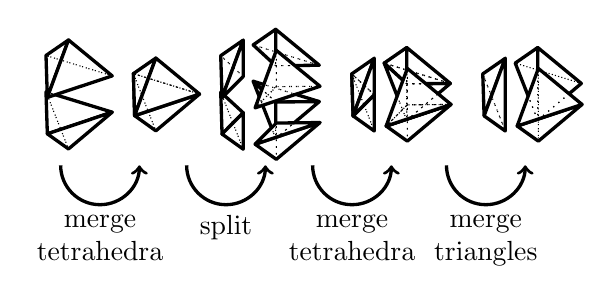
\begin{tikzpicture}[line join=round]
\filldraw[very thick,fill=white](2.631,-.096)--(2.345,.168)--(2.631,-.558)--cycle;
\filldraw[very thick,fill=white](3.185,-.091)--(2.345,.168)--(2.631,-.096)--cycle;
\filldraw[very thick,fill=white](2.631,-.558)--(3.185,-.091)--(2.631,-.096)--cycle;
\filldraw[very thick,fill=white](4.849,.14)--(4.009,.398)--(4.295,.135)--cycle;
\filldraw[very thick,fill=white](4.295,.596)--(4.009,.398)--(4.295,.135)--cycle;
\filldraw[very thick,fill=white](4.295,.135)--(4.009,.398)--(4.295,-.327)--cycle;
\filldraw[very thick,fill=white](5.673,.398)--(5.959,-.327)--(5.959,.596)--cycle;
\filldraw[very thick,fill=white](-.286,.033)--(-.269,-.5)--(.555,-.225)--cycle;
\filldraw[very thick,fill=white](1.933,.03)--(1.95,-.503)--(2.219,-.233)--cycle;
\filldraw[very thick,fill=white](4.295,-.327)--(4.849,.14)--(4.295,.135)--cycle;
\filldraw[very thick,fill=white](5.959,.596)--(5.959,-.327)--(6.513,.14)--cycle;
\filldraw[very thick,fill=white](.555,-.225)--(-.269,-.5)--(0,-.692)--cycle;
\filldraw[very thick,fill=white](2.219,-.233)--(1.95,-.503)--(2.219,-.695)--cycle;
\filldraw[very thick,fill=white](2.631,.827)--(2.345,.629)--(2.631,.365)--cycle;
\filldraw[very thick,fill=white](.824,.264)--(.84,-.269)--(1.664,.005)--cycle;
\filldraw[very thick,fill=white](.824,.264)--(.84,-.269)--(1.109,.462)--cycle;
\filldraw[very thick,fill=white](3.597,.261)--(3.614,-.272)--(3.883,-.003)--cycle;
\filldraw[very thick,fill=white](3.597,.261)--(3.614,-.272)--(3.883,.459)--cycle;
\filldraw[very thick,fill=white](5.261,.261)--(5.278,-.272)--(5.547,.459)--cycle;
\filldraw[very thick,fill=white](1.664,.005)--(.84,-.269)--(1.109,-.462)--cycle;
\filldraw[very thick,fill=white](3.883,-.003)--(3.614,-.272)--(3.883,-.464)--cycle;
\filldraw[very thick,fill=white](5.278,-.272)--(5.547,-.464)--(5.547,.459)--cycle;
\filldraw[very thick,fill=white](3.194,-.357)--(2.37,-.632)--(2.639,-.824)--cycle;
\filldraw[very thick,fill=white](-.286,.495)--(-.269,-.038)--(0,.692)--cycle;
\filldraw[very thick,fill=white](1.933,.492)--(1.95,-.041)--(2.219,.69)--cycle;
\filldraw[very thick,fill=white](4.295,.135)--(4.849,.14)--(4.295,.596)--cycle;
\filldraw[very thick,fill=white](4.858,-.127)--(4.034,-.401)--(4.303,-.593)--cycle;
\filldraw[very thick,fill=white](5.967,-.593)--(6.522,-.127)--(5.698,-.401)--cycle;
\filldraw[very thick,fill=white](2.631,.365)--(3.185,.371)--(2.631,.827)--cycle;
\filldraw[very thick,fill=white](1.109,.462)--(.84,-.269)--(1.664,.005)--cycle;
\filldraw[very thick,fill=white](3.883,.459)--(3.614,-.272)--(3.883,-.003)--cycle;
\filldraw[very thick,fill=white](2.37,-.632)--(3.194,-.357)--(2.639,-.363)--cycle;
\filldraw[very thick,fill=white](0,.692)--(-.269,-.038)--(.555,.236)--cycle;
\filldraw[very thick,fill=white](2.219,.69)--(1.95,-.041)--(2.219,.228)--cycle;
\filldraw[very thick,fill=white](4.034,-.401)--(4.858,-.127)--(4.303,-.132)--cycle;
\filldraw[very thick,fill=white](5.698,-.401)--(6.522,-.127)--(5.967,.33)--cycle;
\filldraw[very thick,fill=white](4.034,-.401)--(4.858,-.127)--(4.303,.33)--cycle;
\filldraw[very thick,fill=white](2.37,-.17)--(3.194,.104)--(2.639,.56)--cycle;
\filldraw[fill=none,dotted](-.286,.495)--(-.269,-.038)--(0,.692)--cycle;
\filldraw[fill=none,dotted](0,.692)--(-.269,-.038)--(.555,.236)--cycle;
\filldraw[fill=none,dotted](.555,.236)--(-.286,.495)--(0,.692)--cycle;
\filldraw[fill=none,dotted](-.269,-.038)--(-.286,.495)--(.555,.236)--cycle;
\filldraw[fill=none,dotted](-.269,-.5)--(-.286,.033)--(0,-.692)--cycle;
\filldraw[fill=none,dotted](0,-.692)--(-.286,.033)--(.555,-.225)--cycle;
\filldraw[fill=none,dotted](.555,-.225)--(-.269,-.5)--(0,-.692)--cycle;
\filldraw[fill=none,dotted](-.286,.033)--(-.269,-.5)--(.555,-.225)--cycle;
\filldraw[fill=none,dotted](.824,.264)--(.84,-.269)--(1.109,.462)--cycle;
\filldraw[fill=none,dotted](1.109,.462)--(.84,-.269)--(1.664,.005)--cycle;
\filldraw[fill=none,dotted](1.664,.005)--(.824,.264)--(1.109,.462)--cycle;
\filldraw[fill=none,dotted](.84,-.269)--(.824,.264)--(1.664,.005)--cycle;
\filldraw[fill=none,dotted](.84,-.269)--(.824,.264)--(1.109,-.462)--cycle;
\filldraw[fill=none,dotted](1.109,-.462)--(.824,.264)--(1.664,.005)--cycle;
\filldraw[fill=none,dotted](1.664,.005)--(.84,-.269)--(1.109,-.462)--cycle;
\filldraw[fill=none,dotted](.824,.264)--(.84,-.269)--(1.664,.005)--cycle;
\filldraw[fill=none,dotted](3.185,.371)--(2.345,.629)--(2.631,.827)--cycle;
\filldraw[fill=none,dotted](2.631,.827)--(2.345,.629)--(2.631,.365)--cycle;
\filldraw[fill=none,dotted](2.631,.365)--(3.185,.371)--(2.631,.827)--cycle;
\filldraw[fill=none,dotted](2.345,.629)--(3.185,.371)--(2.631,.365)--cycle;
\filldraw[fill=none,dotted](1.933,.492)--(1.95,-.041)--(2.219,.69)--cycle;
\filldraw[fill=none,dotted](2.219,.69)--(1.95,-.041)--(2.219,.228)--cycle;
\filldraw[fill=none,dotted](2.219,.228)--(1.933,.492)--(2.219,.69)--cycle;
\filldraw[fill=none,dotted](1.95,-.041)--(1.933,.492)--(2.219,.228)--cycle;
\filldraw[fill=none,dotted](2.37,-.17)--(3.194,.104)--(2.639,.56)--cycle;
\filldraw[fill=none,dotted](2.639,.56)--(3.194,.104)--(2.639,.099)--cycle;
\filldraw[fill=none,dotted](2.639,.099)--(2.37,-.17)--(2.639,.56)--cycle;
\filldraw[fill=none,dotted](3.194,.104)--(2.37,-.17)--(2.639,.099)--cycle;
\filldraw[fill=none,dotted](3.194,-.357)--(2.37,-.632)--(2.639,-.824)--cycle;
\filldraw[fill=none,dotted](2.639,-.824)--(2.37,-.632)--(2.639,-.363)--cycle;
\filldraw[fill=none,dotted](2.639,-.363)--(3.194,-.357)--(2.639,-.824)--cycle;
\filldraw[fill=none,dotted](2.37,-.632)--(3.194,-.357)--(2.639,-.363)--cycle;
\filldraw[fill=none,dotted](1.95,-.503)--(1.933,.03)--(2.219,-.695)--cycle;
\filldraw[fill=none,dotted](2.219,-.695)--(1.933,.03)--(2.219,-.233)--cycle;
\filldraw[fill=none,dotted](2.219,-.233)--(1.95,-.503)--(2.219,-.695)--cycle;
\filldraw[fill=none,dotted](1.933,.03)--(1.95,-.503)--(2.219,-.233)--cycle;
\filldraw[fill=none,dotted](2.345,.168)--(3.185,-.091)--(2.631,-.558)--cycle;
\filldraw[fill=none,dotted](2.631,-.558)--(3.185,-.091)--(2.631,-.096)--cycle;
\filldraw[fill=none,dotted](2.631,-.096)--(2.345,.168)--(2.631,-.558)--cycle;
\filldraw[fill=none,dotted](3.185,-.091)--(2.345,.168)--(2.631,-.096)--cycle;
\filldraw[fill=none,dotted](4.849,.14)--(4.009,.398)--(4.295,.596)--cycle;
\filldraw[fill=none,dotted](4.295,.596)--(4.009,.398)--(4.295,.135)--cycle;
\filldraw[fill=none,dotted](4.295,.135)--(4.849,.14)--(4.295,.596)--cycle;
\filldraw[fill=none,dotted](4.009,.398)--(4.849,.14)--(4.295,.135)--cycle;
\filldraw[fill=none,dotted](3.597,.261)--(3.614,-.272)--(3.883,.459)--cycle;
\filldraw[fill=none,dotted](3.883,.459)--(3.614,-.272)--(3.883,-.003)--cycle;
\filldraw[fill=none,dotted](3.883,-.003)--(3.597,.261)--(3.883,.459)--cycle;
\filldraw[fill=none,dotted](3.614,-.272)--(3.597,.261)--(3.883,-.003)--cycle;
\filldraw[fill=none,dotted](4.034,-.401)--(4.858,-.127)--(4.303,.33)--cycle;
\filldraw[fill=none,dotted](4.303,.33)--(4.858,-.127)--(4.303,-.132)--cycle;
\filldraw[fill=none,dotted](4.303,-.132)--(4.034,-.401)--(4.303,.33)--cycle;
\filldraw[fill=none,dotted](4.858,-.127)--(4.034,-.401)--(4.303,-.132)--cycle;
\filldraw[fill=none,dotted](4.858,-.127)--(4.034,-.401)--(4.303,-.593)--cycle;
\filldraw[fill=none,dotted](4.303,-.593)--(4.034,-.401)--(4.303,-.132)--cycle;
\filldraw[fill=none,dotted](4.303,-.132)--(4.858,-.127)--(4.303,-.593)--cycle;
\filldraw[fill=none,dotted](4.034,-.401)--(4.858,-.127)--(4.303,-.132)--cycle;
\filldraw[fill=none,dotted](3.614,-.272)--(3.597,.261)--(3.883,-.464)--cycle;
\filldraw[fill=none,dotted](3.883,-.464)--(3.597,.261)--(3.883,-.003)--cycle;
\filldraw[fill=none,dotted](3.883,-.003)--(3.614,-.272)--(3.883,-.464)--cycle;
\filldraw[fill=none,dotted](3.597,.261)--(3.614,-.272)--(3.883,-.003)--cycle;
\filldraw[fill=none,dotted](4.009,.398)--(4.849,.14)--(4.295,-.327)--cycle;
\filldraw[fill=none,dotted](4.295,-.327)--(4.849,.14)--(4.295,.135)--cycle;
\filldraw[fill=none,dotted](4.295,.135)--(4.009,.398)--(4.295,-.327)--cycle;
\filldraw[fill=none,dotted](4.849,.14)--(4.009,.398)--(4.295,.135)--cycle;
\filldraw[fill=none,dotted](5.673,.398)--(5.959,-.327)--(5.959,.596)--cycle;
\filldraw[fill=none,dotted](5.959,.596)--(5.959,-.327)--(6.513,.14)--cycle;
\filldraw[fill=none,dotted](6.513,.14)--(5.673,.398)--(5.959,.596)--cycle;
\filldraw[fill=none,dotted](5.959,-.327)--(5.673,.398)--(6.513,.14)--cycle;
\filldraw[fill=none,dotted](5.278,-.272)--(5.547,-.464)--(5.547,.459)--cycle;
\filldraw[fill=none,dotted](5.547,.459)--(5.547,-.464)--(5.261,.261)--cycle;
\filldraw[fill=none,dotted](5.261,.261)--(5.278,-.272)--(5.547,.459)--cycle;
\filldraw[fill=none,dotted](5.547,-.464)--(5.278,-.272)--(5.261,.261)--cycle;
\filldraw[fill=none,dotted](6.522,-.127)--(5.967,-.593)--(5.967,.33)--cycle;
\filldraw[fill=none,dotted](5.967,.33)--(5.967,-.593)--(5.698,-.401)--cycle;
\filldraw[fill=none,dotted](5.698,-.401)--(6.522,-.127)--(5.967,.33)--cycle;
\filldraw[fill=none,dotted](5.967,-.593)--(6.522,-.127)--(5.698,-.401)--cycle;

\begin{scope}[very thick]
    \draw[->] (-0.1, -0.9) arc[start angle=180, end angle=360, radius=0.5] node[midway, below, align=center] {merge\\tetrahedra};
    \draw[->] (1.5, -0.9) arc[start angle=180, end angle=360, radius=0.5] node[midway, below, align=center] {split};
    \draw[->] (3.1, -0.9) arc[start angle=180, end angle=360, radius=0.5] node[midway, below, align=center] {merge\\tetrahedra};
    \draw[->] (4.8, -0.9) arc[start angle=180, end angle=360, radius=0.5] node[midway, below, align=center] {merge\\triangles};
\end{scope}
\end{tikzpicture}% End sketch output

    \end{center}
    \caption{A 2-3 flip implemented as a sequence of merges and splits.
    We've shown the tetrahedra in an ``exploded'' view to help with visualization.}
    \label{fig:2-3-flip}
\end{figure}



% =====================
\section{Demonstration}

As a proof of concept, we developed a software package called \emph{topomesh} which implements the transformations defined above.
We then implemented several common algorithms in computational geometry using these transformations.

% -------------------------------------
\subsection{Convex hulls and vertex-split}

The vertex-split transformation is the key computational kernel for computing convex hulls in any dimension.
The source code for the vertex-split transformation is shown in figure \ref{fig:split-source-code}.
\begin{figure}
    \begin{minted}[fontsize=\footnotesize,linenos]{python}
import numpy as np
from typing import List

Topology = List[np.ndarray]

def vertex_split(D: Topology) -> Topology:
    # Create the boundary matrices for 1 <= k < n
    n_vertices = D[0].shape[1]
    E = [np.ones((1, n_vertices + 1), int)]
    for k in range(1, len(D) - 1):
        n_cells = D[k].shape[1]
        n_sub_faces, n_faces = D[k - 1].shape
        I = np.identity(n_faces, int)
        Z = np.zeros((n_sub_faces, n_cells), int)
        E_k = np.block([[D[k], I], [Z, -D[k - 1]]])
        E.append(E_k)

    # Create the top-dimensional boundary matrix
    C = np.diag(np.sum(D[-1], axis=1))
    E_n = np.vstack((C, -D[-2] @ C))
    E.append(E_n)
    return E
    \end{minted}
    \caption{Python source code for the split transformation.
    Line 15 corresponds to equation \eqref{eq:cone-partial-k}; lines 19-20 correspond to equation \eqref{eq:vertex-split-n}.
    The real version has some additional logic to remove empty cells.}
    \label{fig:split-source-code}
\end{figure}

We used the split transformation to implement a convex hull algorithm that works in arbitrary dimensions.
To test the convex hull code, we used (1) random point sets up to dimension 5 and (2) several synthetic input sets with various degeneracies such as coplanarity.
For geometric predicates, we first compute the determinant using interval arithmetic; if the result interval contains zero, we try again with exact rationals.

Our implementation of the convex hull algorithm takes in a function as argument which supplies the procedure for computing the signed volume predicate.
Computing Delaunay triangulations is equivalent to computing the lower half of a convex hull of the input points lifted to a paraboloid.
We also implemented a Delaunay triangulation method which reuses our convex hull algorithm by supplying an insphere function instead of the usual signed volume function.

% ---------------------------------------------------
\subsection{Constrained Delaunay triangulation and face-split}

\begin{figure}[t]
    \begin{center}
        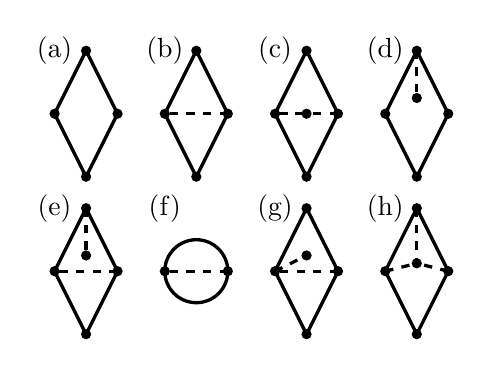
\begin{tikzpicture}[scale=0.4]
    \newcommand*{\defcoords}{
        \coordinate (p0) at (1, 0){};
        \coordinate (p1) at (0, 2){};
        \coordinate (p2) at (-1, 0){};
        \coordinate (p3) at (0, -2){};

        \begin{scope}[very thick]
            \draw (p0) -- (p1) -- (p2) -- (p3) -- cycle;
            \foreach \p in {p0, p1, p2, p3} {
                \filldraw (\p) circle (3pt);
            }
        \end{scope}

    }

    \begin{scope}[very thick]
        \defcoords 
        \node[] at (-1, 2) {(a)};
    \end{scope}

    \begin{scope}[very thick, shift={(3.5, 0)}]
        \defcoords
        \node[] at (-1, 2) {(b)};
        \draw[dashed] (p0) -- (p2);
    \end{scope}

    \begin{scope}[very thick, shift={(7.0, 0)}]
        \defcoords
        \node[] at (-1, 2) {(c)};
        \coordinate (p4) at (0, 0){};
        \filldraw (p4) circle (3pt);
        \draw[dashed] (p0) -- (p2) -- (p4);
    \end{scope}

    \begin{scope}[very thick, shift={(10.5, 0)}]
        \defcoords
        \node[] at (-1, 2) {(d)};
        \coordinate (p4) at (0, 0.5){};
        \filldraw (p4) circle (3pt);
        \draw[dashed] (p1) -- (p4);
    \end{scope}

    \begin{scope}[very thick, shift={(0, -5)}]
        \node[] at (-1, 2) {(e)};
        \defcoords
        \draw[dashed] (p0) -- (p2);
        \coordinate (p4) at (0, 0.5){};
        \filldraw (p4) circle (3pt);
        \draw[dashed] (p1) -- (p4);
    \end{scope}

    \begin{scope}[very thick, shift={(3.5, -5)}]
        \node[] at (-1, 2) {(f)};
        \coordinate (p0) at (0, 0){};
        \coordinate (p1) at (1, 0){};
        \coordinate (p2) at (-1, 0){};
        \filldraw (p1) circle (3pt);
        \filldraw (p2) circle (3pt);
        \draw[dashed] (p1) -- (p2);
        \draw[fill=none](p0) circle (1.0) {};
    \end{scope}

    \begin{scope}[very thick, shift={(7.0, -5)}]
        \defcoords
        \node[] at (-1, 2) {(g)};
        \draw[dashed] (p0) -- (p2);
        \coordinate (p4) at (0, 0.5){};
        \filldraw (p4) circle (3pt);
        \draw[dashed] (p2) -- (p4);
    \end{scope}

    \begin{scope}[very thick, shift={(10.5, -5)}]
        \defcoords
        \node[] at (-1, 2) {(h)};
        \coordinate (p4) at (0, 0.25){};
        \filldraw (p4) circle (3pt);
        \draw [dashed] (p0) -- (p4);
        \draw [dashed] (p1) -- (p4);
        \draw [dashed] (p2) -- (p4);
    \end{scope}

\end{tikzpicture}

    \end{center}
    \caption{Test cases for splitting polygons along edges: (a) nothing to split at all, (b) splitting along an edge, (c) splitting along multiple edges, (d) nothing to split but with a hanging face, (e) splitting along an edge but with a hanging face, (f) straightforward split but with linearly dependent columns of $\partial_1$, (g) extraneous hanging edge, (h) three-way split.}
    \label{fig:face-split-tests}
\end{figure}

The vertex-split transformation alone is enough to compute convex hulls and unconstrained Delaunay triangulations.
Computing a constrained Delaunay triangulation (CDT) additionally requires merges and face-splits.

A significant complication that can arise in computing the CDT is the presence of \emph{hanging edges} \cite{cheng2013delaunay}.
Inserting a constrained edge into a CDT requires forming the polygonal cavity consisting of the union of all the triangles that the constrained edge passes through.
The constrained edge is then inserted, dividing the polygonal cavity in two.
The remaining two polygonal cavities are then repeatedly subdivided until only triangles remain.
Now, the initial cavity formation can create a hanging edge.
In this instance we know that the separator consists only of the constrained edge.
At some later step, the hanging edge will be connected by two more edges and become part of the separator.
In short, we can assume that at least one face of the separator is known from the outset, but not that we know the entire separator.
Our implementation uses a breadth-first search to identify the entire separator from the starting faces.
We then perform further searches to mark the remaining connected components.

We first implemented the face-split transformation and tested it on several cases including ones with hanging edges.
The test cases we chose are shown in Figure \ref{fig:face-split-tests}.
Some of these cases should never show up in real problems, but we check for them anyway in the interest of completeness.
Case (h), with only two out of the three separator edges known to start, is the scenario where a hanging edge is incorporated into a CDT.

\begin{figure}
    \begin{center}
    \includegraphics[width=0.98\linewidth]{figures/retria.pdf}
    \end{center}
    \caption{The steps of the cavity retriangulation algorithm.
    The hanging edge at the start and the non-simplicial intermediate states are all representable as boundary operators.}
    \label{fig:cheng-dey-shewchuk-example}
\end{figure}

We then tested several realistic configurations for cavity retriangulation.
Figure \ref{fig:cheng-dey-shewchuk-example} shows one such test case from Figure 3.13 of \cite{cheng2013delaunay}.
This test case is a non-convex cavity with a hanging edge.
The algorithm proceeds entirely by subdividing polygons into smaller ones with no special cases to handle hanging edges beyond the breadth-first searches described above.
By contrast, the CavityCDT algorithm described in \cite{cheng2013delaunay} requires special cases to re-traverse hanging edges and to delete triangles of the wrong orientation.

We implemented a CDT algorithm based on \cite{anglada1997improved}.
\textcolor{red}{Elaborate...}

% -------------------------------------
\subsection{Multi-face retriangulation}

Finally, we implemented part of the multi-face retriangulation described in \cite{misztal2009tetrahedral}.
This transformation is assumed to operate on the suspension of a set of filling triangles.
In \cite{misztal2009tetrahedral}, the filling triangles are identified via a search procedure and are then transformed into another triangulation of the same polygon using Klincsek's algorithm \cite{klincsek1980minimal}.
Here we focus entirely on the transformation step and assume that we are given both the filling triangles and the tetrahedra that they fill.
The goal is to take the suspension $S_1$ of a set of triangles and replace it with the suspension $S_2$ of a given set of triangles $T_2$.

The Python source code for our implementation is shown in Figure \ref{fig:mfrt-code}.
The key features of the topomesh library that this code uses are:
\begin{description}
    \item[\texttt{closure}]: given a set of $k$-cells $\{\sigma_\alpha\}$, return all their immediate faces, their faces' faces, and so on
    \item[\texttt{subcomplex}]: given a set of cells $\{\sigma_\alpha^k\}$, return the boundary matrices corresponding to the subcomplex formed by these cells
    \item[\texttt{find\_isomorphism}]: given a pair of complexes, find the permutations and sign flips that transform one into the other.
\end{description}
We tested the implementation by repeatedly generating two random triangulations of a polygon of $n$ vertices for $n = 4, 5, \ldots, 10$.
We form the suspension of the first set of triangles and apply a random permutation and sign flip.
The test is to see whether we can match its boundary to the boundary of the suspension of the second triangulation.

\begin{figure}[t]
\begin{minted}[fontsize=\footnotesize,linenos]{python}
import numpy as np
from topomesh import polygonal
Topology = list[np.ndarray]

def boundary_complex(T: Topology) -> Topology:
    num_cells = T[-1].shape[1]
    C = T[-1] @ np.ones(num_cells)
    face_ids = np.flatnonzero(C)
    cell_ids = polygonal.closure(T[:-1], face_ids)
    return polygonal.subcomplex(T[:-1], cell_ids)

def retriangulate(
    S_1: Topology,
    T_2: Topology,
) -> Topology:
    dS_1 = boundary_complex(S_1)
    S_2 = polygonal.join_vertices(T_2)
    dS_2 = boundary_complex(S_2)
    return polygonal.find_isomorphism(dS_1, dS_2)
\end{minted}
    \caption{Source code for multi-face retriangulation.}
\label{fig:mfrt-code}
\end{figure}


% ==================
\section{Conclusion}

Doubly-connected edge lists have historically been popular for mesh generation because they offer a simple interface for traversing the topology \cite{guibas1985primitives}.
Here we propose that boundary operators are a viable choice of representation if the goal is to perform topological transformations.
This idea has appeared before, for example in the work of DiCarlo and others \cite{dicarlo2007solid}.

Boundary operators are only necessary for representing a small patch of the topology at a time.
Once the transformed patch is computed, it can be translated back to a set of simplices.
Boundary operators are useful for describing non-simplicial intermediate states of a transformation; they are not space-optimal for describing an entire simplicial complex.

We showed how to implement two common topological operations for tetrahedral mesh improvement.
These operations assume a particular structure for the tetrahedra that they operate on.
The \emph{small polyhedron reconnection} (SPR) approach, by contrast, works on any set of input tetrahedra at the cost of a more expensive search step \cite{marot2020reviving}.
The linear algebraic representation may have the potential to accelerate small polyhedron reconnection or other approaches to tetrahedral mesh improvement.
If reasonable polytope quality measures can be defined, it may instead be possible to search for optimal tetrahedralizations by iteratively bisecting the cavity into smaller polytopes that do not need to be simplicial until the end.

We checked that the constructions defined here work as expected by testing that we could compute convex hulls, Delaunay triangulations, etc.
We did not give formal proofs that each operation is guaranteed to result in a topologically valid end state given certain preconditions.
For example, applying the face-split transformation assumes that a certain integer linear system is solvable.
Are there cases where this system has either no solution or multiple solutions despite the fact that the polytope is splittable?
Are there cases where the system does have a unique solution but not one that produces the desired final topology?
We found empirically that the linear system was solvable in all the cases that we tried and gave the expected results.
But an interesting future direction would be to use formal methods to verify these transformations using established results, for example on total unimodularity of boundary matrices \cite{dey2010optimal}.

When the objects of study can be represented as linear operators, we can apply linear algebraic reasoning to define transformations and verify that they preserve all of the important invariants.
The condition in equation \eqref{eq:ddzero} that the product of two boundary operators is zero is a powerful invariant for ensuring the validity of the underlying topology.


\bibliography{chain-complexes.bib}

\end{document}
